\section{Models}

We implemented the RSP formulation ideas above on a simple aircraft design problem as defined in~\cite{Ozturk2018}.
We conduct optimization of a wing, fuselage, engine given a payload and range requirement.

A short overview of the model

\subsection{Flight Profile}

The flight trajectory of the aircraft is optimized

\subsection{Atmosphere Model}

The atmosphere model

\subsection{Wing Model}

\subsection{Fuselage Model}



\subsection{Engine Model}

The aircraft is powered by a naturally aspirated piston engine. This means that it is subject to the


\subsection{Lift, Weight, Drag and Thrust}

The weight of the aircraft is the sum of the payload weight, wing weight, and
the fuselage weight, as shown in Figure~\ref{fig:liftweight}. Lift is generated by the wing,
which is described by an aspect ratio $\AR$ and surface area $S$.

\begin{figure}
\centering
\caption{\label{fig:liftweight} Wing lift is equal and opposite to the wing weight, payload weight, and total fuel weight.}
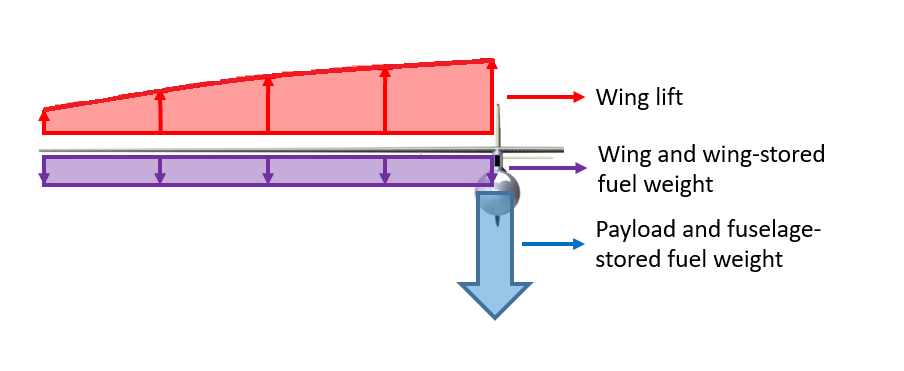
\includegraphics[width=0.8\textwidth]{liftweight.PNG}
\end{figure}

\subsection{Wing Structure}
The wing structure model is based on a simple beam model with a distributed lift load,
and a point mass in the center representing the fuselage, as shown in Figure~\ref{fig:liftweight}.

\subsection{Fuel Volume}
The fuel in the aircraft can be stored either in the wing or the fuselage.
The signomial constraint in the optimization appears in the fuel volume model, as shown in Equation~\ref{eq:fuel}:

\begin{equation}
\label{eq:fuel}
V_f \leq V_{f_{wing}} + V_{f_{fuse}} 
\end{equation}

where $V_{f_{wing}}$ and $V_{f_{fuse}}$ represent the fuel volume available in the wing
and the fuselage respectively. They are each represented by the following monomials.

\begin{equation}
\label{eq:fuelwing}
V_{f_{wing}} \leq 9 \times 10^{-4} \frac{S^{1.5}\tau}{A^{0.5}}
\end{equation}

\begin{equation}
\label{eq:fuelfuse}
V_{f_{fuse}} \leq 10 \times \CDA_0~m
\end{equation}

Note that the monomials above are represented with inequalities, to be compatible with the RSP formulation. 

\subsection{Takeoff constraints}
We specify that the aircraft has to be able to takeoff at a speed of $V_{min}$
without exceeding the aircraft stall lift coefficient $C_{L_{max}}$, both of which are
specified with an associated uncertainty.
